%! TEX root = main.tex
The overall run times for the steady, unsteady, and data-driven cases are about 28 hours, 31 hours, and 33.5 hours.
The PetIBM simulation, on the other hand, took around 1.7 hours with a 5-generation-behind GPU.

Figure \ref{fig:cylinder-re200-train-hist} shows the convergence history of all cases.
\begin{figure}[hbt!]
    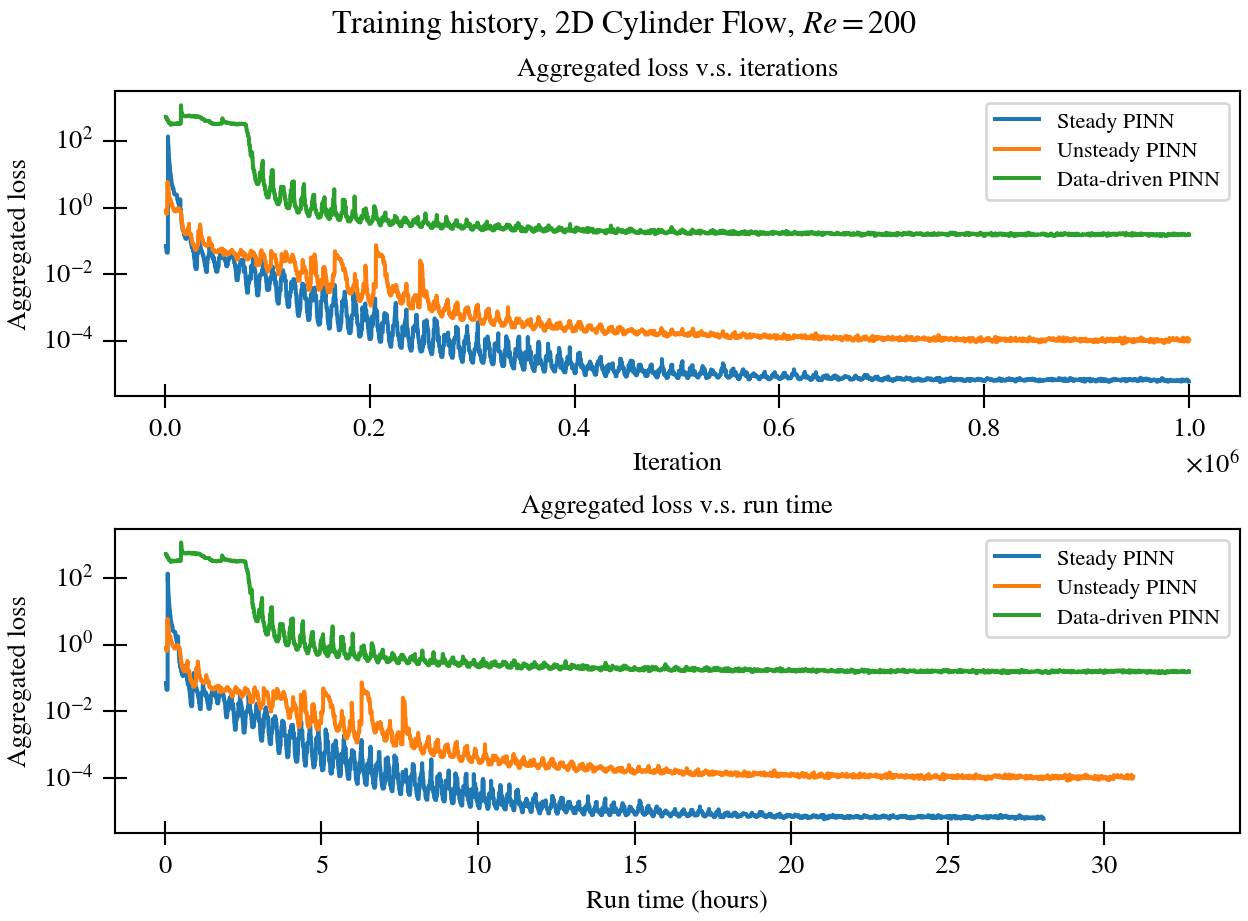
\includegraphics[width=0.9\linewidth]{cylinder-2d-re200/loss-hist}
    \caption{PINNs, 2D Cylinder, $Re=200$: training history}
    \label{fig:cylinder-re200-train-hist}
\end{figure}
One sub-plot is for losses versus iterations, while the other one is against the run times.
The plateaus we observed in the $Re=40$ cases also exist in the unsteady and data-driven cases here.
The steady case does not show any sign of the plateau.
The data-driven case does not converge to a loss level as small as that of the other two cases.
However, the aggregated loss of the data-driven case has extra data loss terms, so it is unclear at this point if all loss terms have higher values or only the data loss terms are higher. 

\begin{table}[hbt!]
    \singlespacing
    \begin{threeparttable}[b]
        \begin{tabular}{lcc}
            \toprule
            & $C_D$ \\
            \midrule
            PetIBM & 1.38   \\
            Steady PINN & 0.95 \\
            Unsteady PINN & 0.95 \\
            Deng et al., 2007\cite{deng_hydrodynamic_2007}\tnote{1} & 1.25 \\
            Rajani et al., 2009\cite{Rajani2009}\tnote{1} & 1.34 \\
            Gushchin \& Shchennikov, 1974\cite{gushchin_numerical_1974}\tnote{2} & 0.97 \\
            Fornberg, 1980\cite{fornberg_numerical_1980}\tnote{2} & 0.83 \\
            \bottomrule
        \end{tabular}%
        \begin{tablenotes}
            \footnotesize
            \item [1] Unsteady simulations.
            \item [2] Steady simulations.
        \end{tablenotes}
        \caption[
            PINNs, 2D Cylinder, $Re=200$: validation of drag coefficients%
        ]{%
            PINNs, 2D Cylinder, $Re=200$: validation of drag coefficients.%
            The data-driven case is excluded because it does not have an obvious periodic state nor a steady-state solution.%
        }%
        \label{table:cylinder-2d-re200-cd}
    \end{threeparttable}
\end{table}%


\begin{figure}[hbt!]
    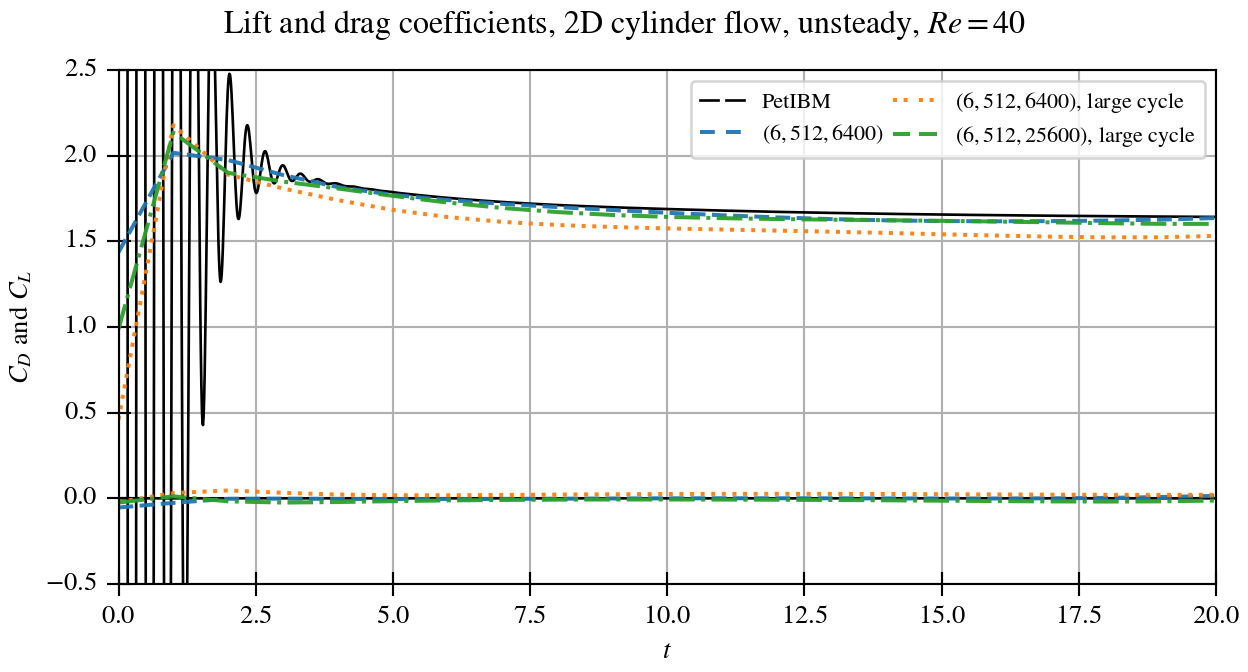
\includegraphics[width=0.9\linewidth]{cylinder-2d-re200/drag-lift-coeffs}
    \caption{PINNs, 2D Cylinder, $Re=200$: drag and lift coefficients}
    \label{fig:cylinder-re200-drag-lift}
\end{figure}

Figure \ref{fig:cylinder-re200-drag-lift} shows the drag and lift coefficients versus simulation time.
The coefficients from the steady case is just a horizontal line because there is no time variable in this case.
The unsteady case, to our surprise, does not exhibit oscillation, meaning probably no vortex shedding.
Although, it fits well with the PetIBM result before shedding happens (before around $t=75$), including the wake development stage before $t=25$.
Comparing the coefficients between the steady, unsteady, and PetIBM's values before shedding, we believe the unsteady PINN in this particular case behaves just like a steady solver.
This speculation is further supported by the values in table \ref{table:cylinder-2d-re200-cd}, where we compare $C_D$ to both unsteady and steady numerical simulations from literature.
The $C_D$ obtained from the unsteady PINN is the same as the steady PINN and close to those steady CFD simulation results.

As for the data-driven case, its temporal domain is $t\in[125$, $200]$, so the coefficients' trajectories start from $t=125$.
The result, again unexpected to us, only exhibits shedding in the time range where we provide data with shedding to the PINN ($t\in[125$, $140]$).
This result also shows that data-driven PINNs may be more difficult to train, compared to data-free PINNs and regular data-only model fitting.
Even in the range of provided data, the data-driven case is not able to reach the given maximal $C_L$, and the $C_D$ is obviously off from the given data.
After $t=140$, the trajectories quickly fall back to the no-shedding pattern, though it still deviates from the trajectories of the steady and unsteady PINNs.
Combining the loss magnitude shown in figure \ref{fig:cylinder-re200-train-hist}, the deviation of values may be caused by not enough training.
As figure \ref{fig:cylinder-re200-train-hist} shows data-driven PINN is converged, other optimization techniques or hyperparameter tuning may be required to further reduce the loss.

Nevertheless, we believe not being trained enough only explains why the data-driven case deviates from the given data and the trajectories of the other two cases.
Even with a better optimization and eventually a lower loss, based on the trajectories, we do not believe the shedding will continue after $t=140$.

To examine how the transient flow develops, below we show several snapshots of the flow fields from PetIBM and PINNs:
\begin{enumerate}
    \item Figure \ref{fig:cylinder-re200-contour-steady} shows the flow field obtained from the steady PINN as a reference.
    \item Figures \ref{fig:cylinder-re200-contour-uv-t10} and \ref{fig:cylinder-re200-contour-pwz-t10}: flow at $t=10$. We can see the wake is still developing, and the unsteady PINN visually matches PetIBM. It means the unsteady PINN is indeed an unsteady solver. This time is out of the data-driven PINN's temporal domain.
    \item Figures \ref{fig:cylinder-re200-contour-uv-t50} and \ref{fig:cylinder-re200-contour-pwz-t50}: flow at $t=50$. These figures further confirm that the unsteady PINN matches the PetIBM simulation before shedding.
    \item Figures \ref{fig:cylinder-re200-contour-uv-t140} and \ref{fig:cylinder-re200-contour-pwz-t140}: flow at $t=140$. At this point, the shedding already happened. And $t=140$ is the last snapshot we fed to the data-driven PINN for training. The flow from data-driven PINN shows that it at least is able to qualitatively capture the shedding, which is expected.
    \item Figures \ref{fig:cylinder-re200-contour-uv-t144} and \ref{fig:cylinder-re200-contour-pwz-t144}: flow at $t=144$. Just $4$ unit time from the last snapshot we fed to the data-driven PINN, the data-driven PINN has already stopped generating new vortices. The existing vortex can be seen moving toward the boundary, and the wake is gradually recovering to the steady state wake.
    \item Figures \ref{fig:cylinder-re200-contour-uv-t190} and \ref{fig:cylinder-re200-contour-pwz-t190}: flow at $t=190$. Flow field at this time further confirms that the data-driven PINN's behavior is leaning toward that of the unsteady PINN, which is itself behaving like a steady state solver.
\end{enumerate}

\begin{figure}[hbt!]
    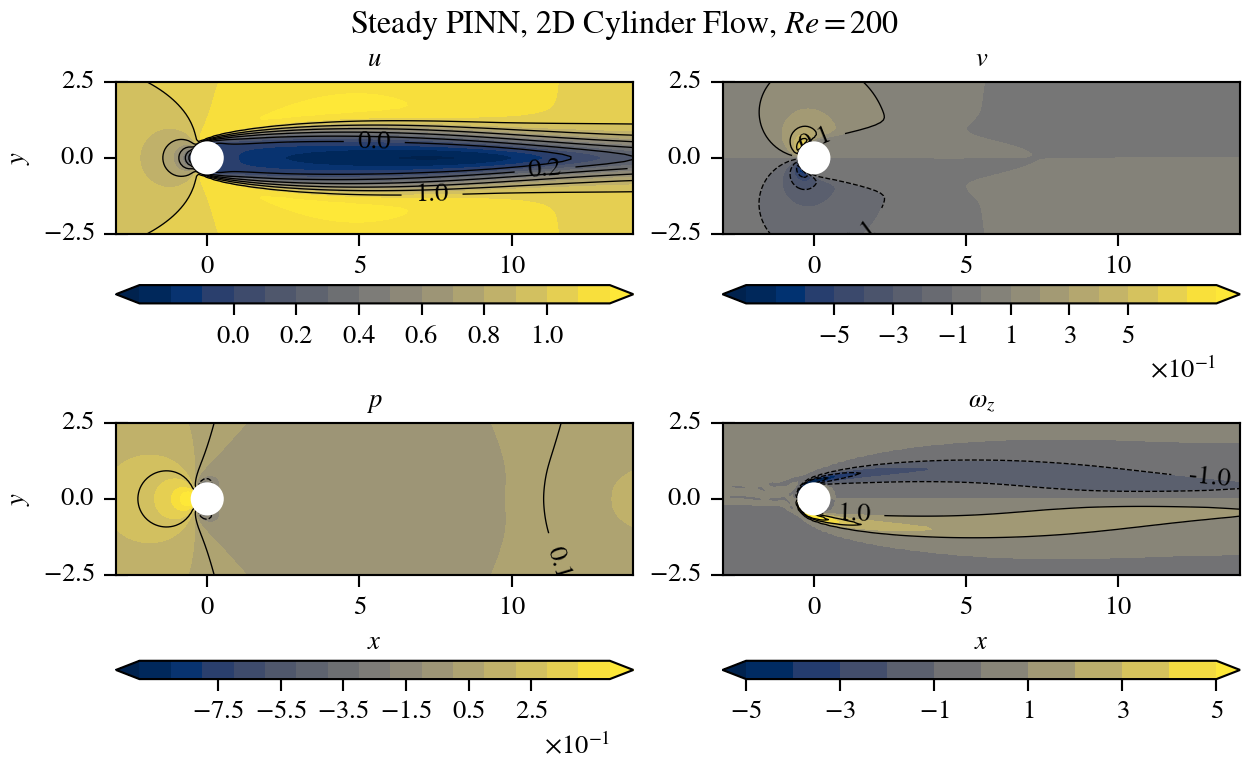
\includegraphics[width=0.9\linewidth]{cylinder-2d-re200/contour-comparison-steady}
    \caption{2D Cylinder, $Re=200$: flow field contours for steady PINN}
    \label{fig:cylinder-re200-contour-steady}
\end{figure}

\begin{figure}[hbt!]
    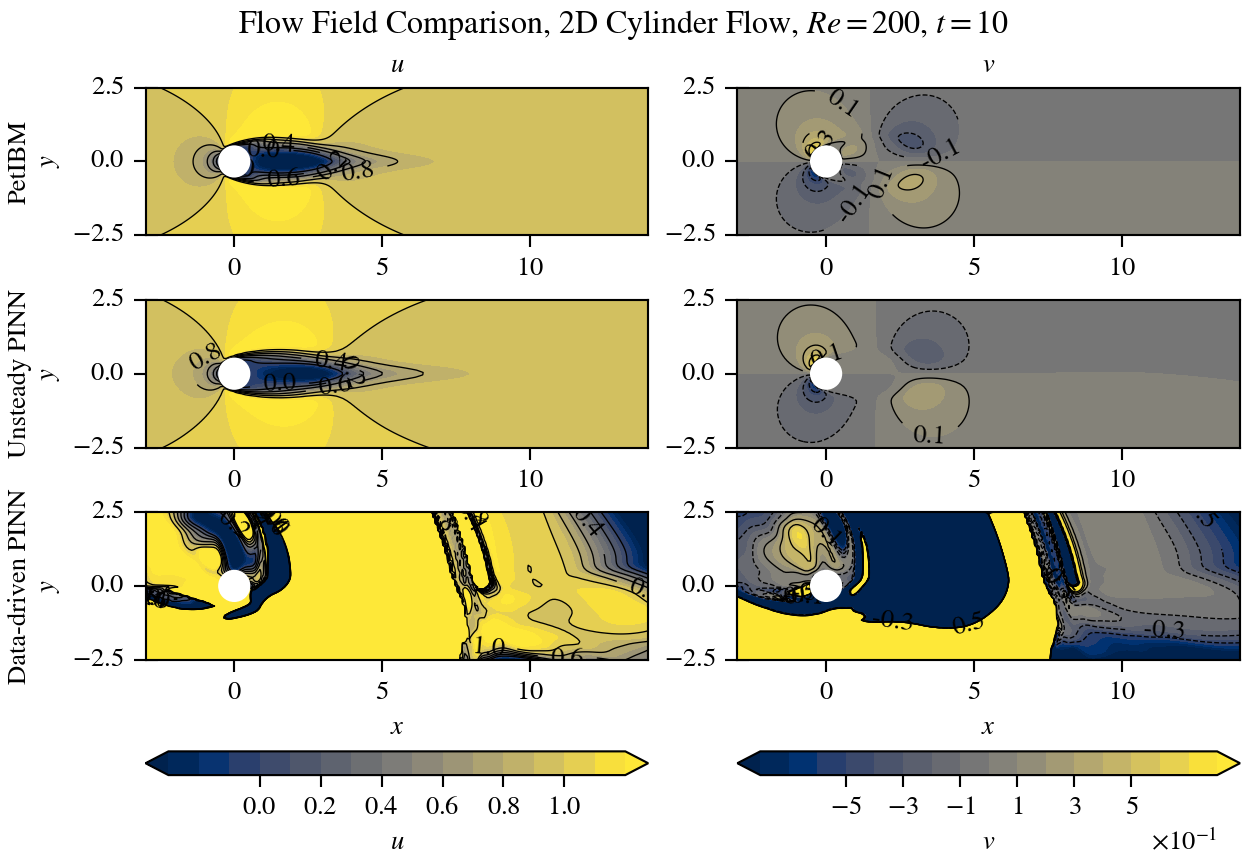
\includegraphics[width=0.9\linewidth]{cylinder-2d-re200/contour-comparison-uv-t10}
    \caption{2D Cylinder, $Re=200$: flow field comparisons for $u$ and $v$ at $t=10$ (PetIBM, data-driven PINN, and data-free PINN)}
    \label{fig:cylinder-re200-contour-uv-t10}
\end{figure}

\begin{figure}[hbt!]
    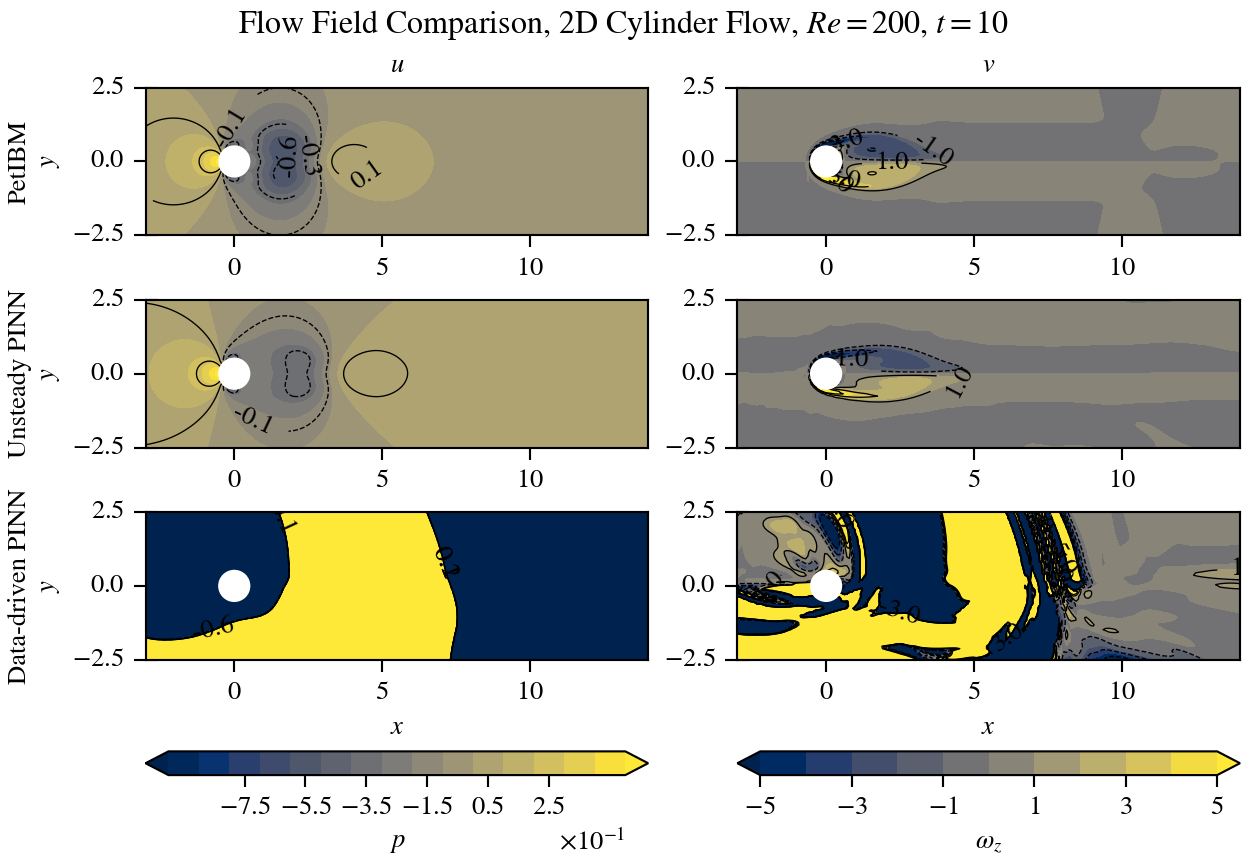
\includegraphics[width=0.9\linewidth]{cylinder-2d-re200/contour-comparison-pwz-t10}
    \caption{2D Cylinder, $Re=200$: flow field comparisons for $p$ and $\omega_z$ at $t=10$ (PetIBM, data-driven PINN, and data-free PINN)}
    \label{fig:cylinder-re200-contour-pwz-t10}
\end{figure}

\begin{figure}[hbt!]
    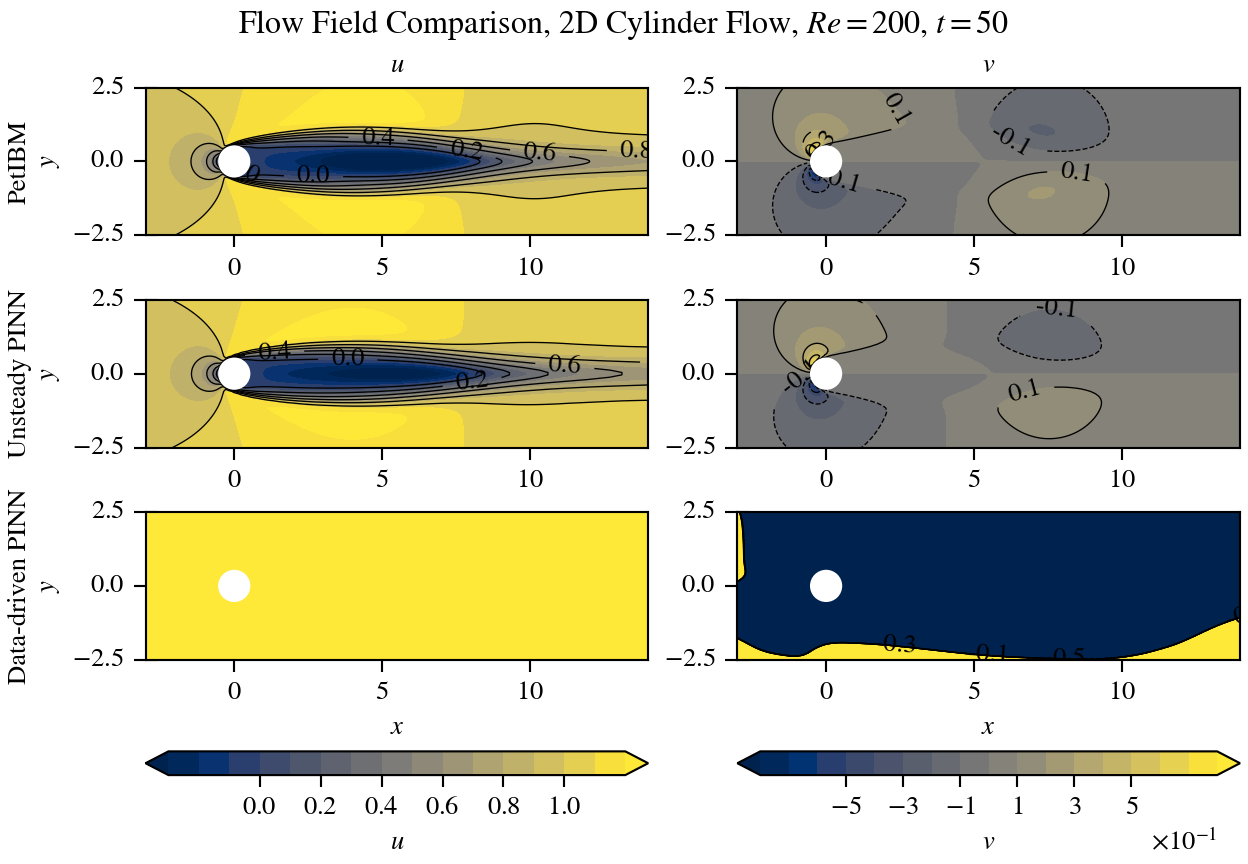
\includegraphics[width=0.9\linewidth]{cylinder-2d-re200/contour-comparison-uv-t50}
    \caption{2D Cylinder, $Re=200$: flow field comparisons for $u$ and $v$ at $t=50$ (PetIBM, data-driven PINN, and data-free PINN)}
    \label{fig:cylinder-re200-contour-uv-t50}
\end{figure}

\begin{figure}[hbt!]
    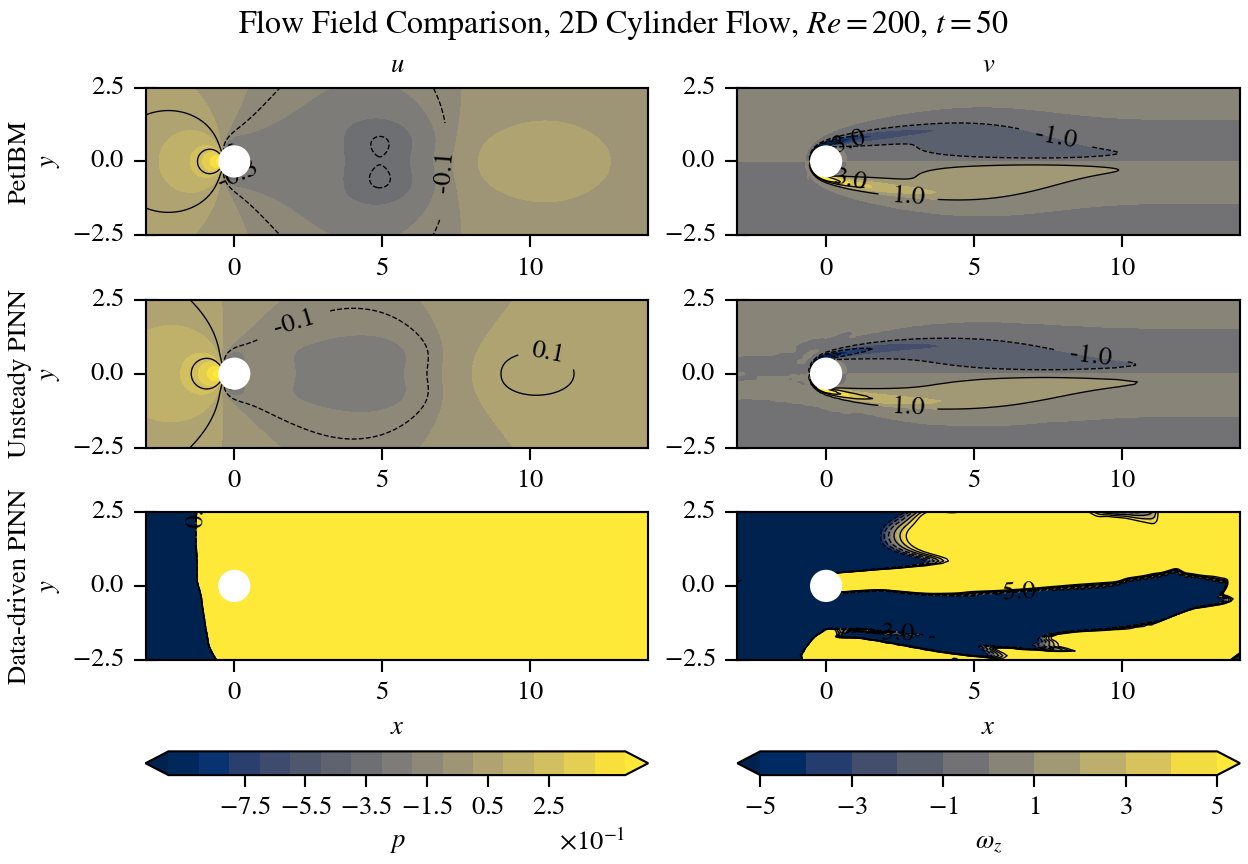
\includegraphics[width=0.9\linewidth]{cylinder-2d-re200/contour-comparison-pwz-t50}
    \caption{2D Cylinder, $Re=200$: flow field comparisons for $p$ and $\omega_z$ at $t=50$ (PetIBM, data-driven PINN, and data-free PINN)}
    \label{fig:cylinder-re200-contour-pwz-t50}
\end{figure}

\begin{figure}[hbt!]
    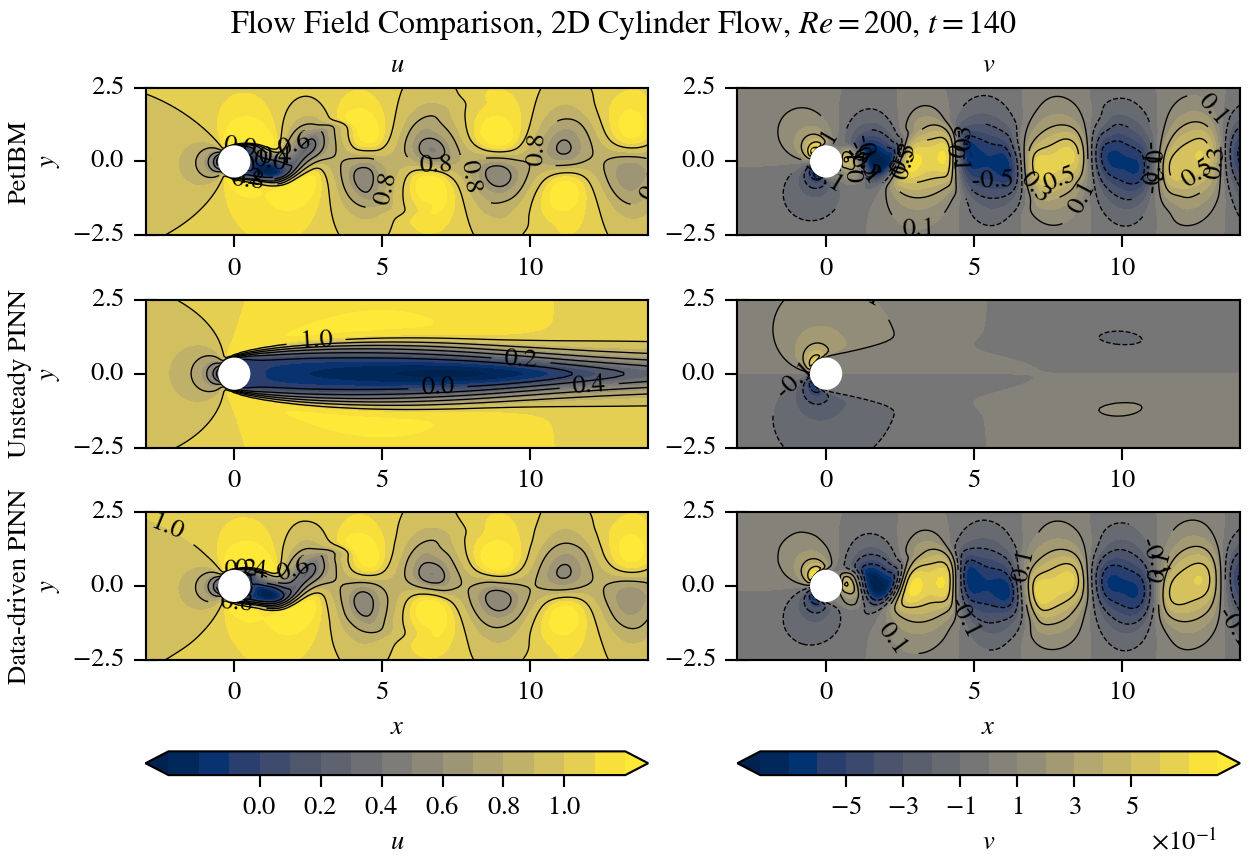
\includegraphics[width=0.9\linewidth]{cylinder-2d-re200/contour-comparison-uv-t140}
    \caption{2D Cylinder, $Re=200$: flow field comparisons for $u$ and $v$ at $t=140$ (PetIBM, data-driven PINN, and data-free PINN)}
    \label{fig:cylinder-re200-contour-uv-t140}
\end{figure}

\begin{figure}[hbt!]
    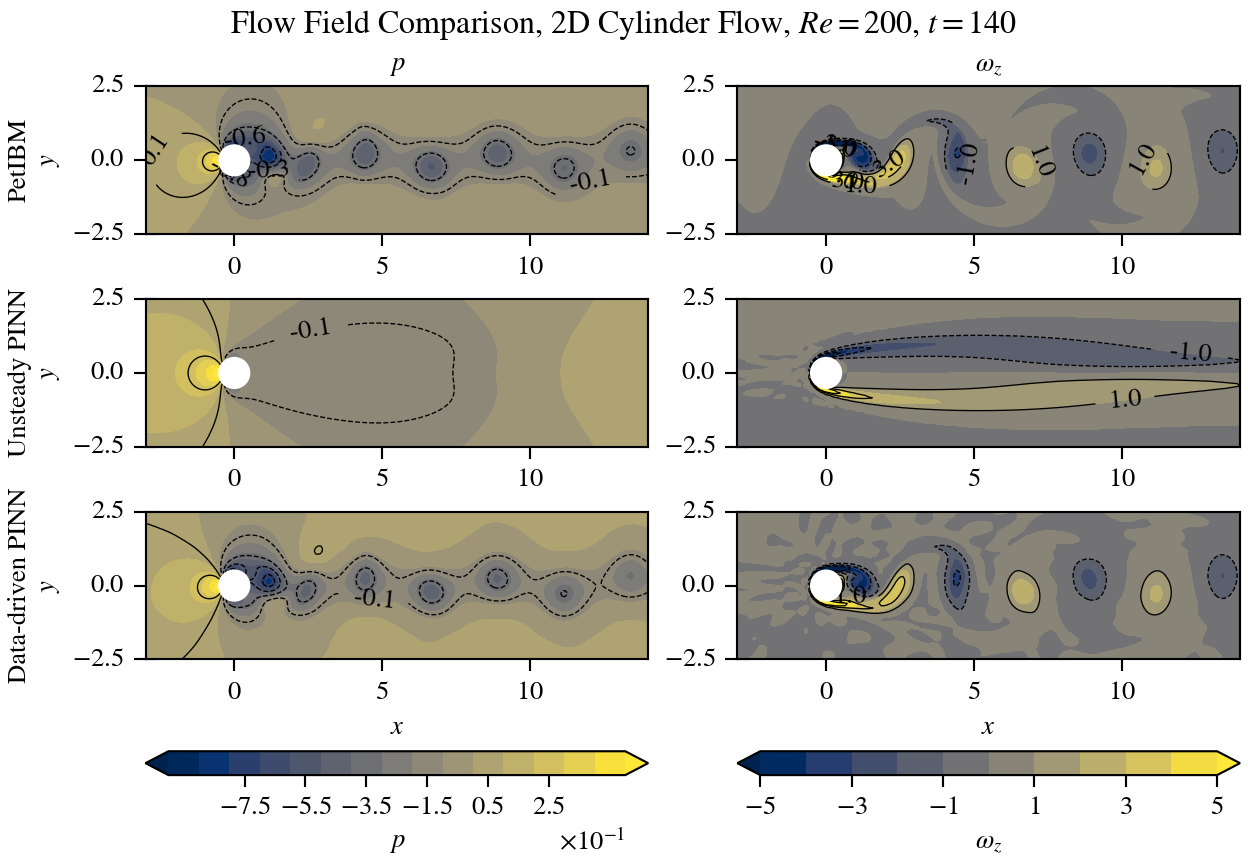
\includegraphics[width=0.9\linewidth]{cylinder-2d-re200/contour-comparison-pwz-t140}
    \caption{2D Cylinder, $Re=200$: flow field comparisons for $p$ and $\omega_z$ at $t=140$ (PetIBM, data-driven PINN, and data-free PINN)}
    \label{fig:cylinder-re200-contour-pwz-t140}
\end{figure}

\begin{figure}[hbt!]
    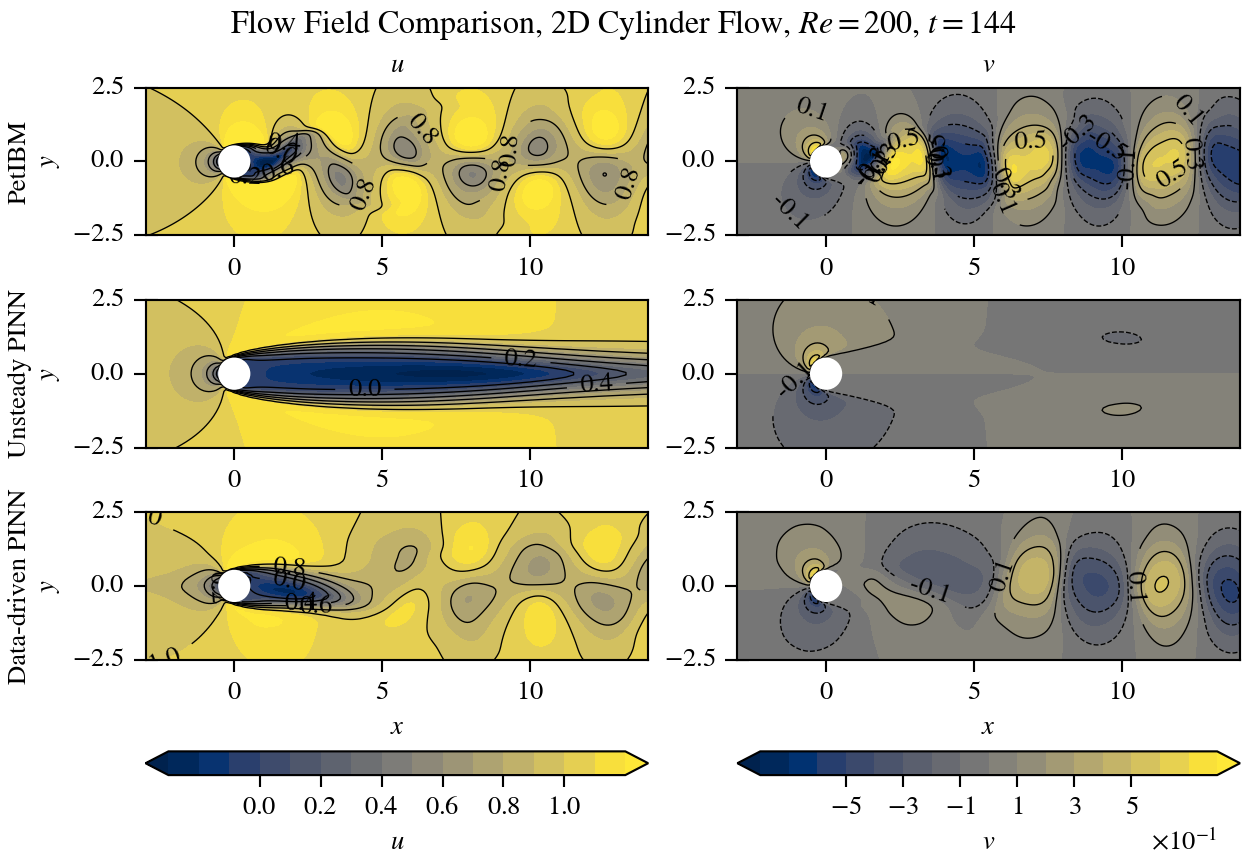
\includegraphics[width=0.9\linewidth]{cylinder-2d-re200/contour-comparison-uv-t144}
    \caption{2D Cylinder, $Re=200$: flow field comparisons for $u$ and $v$ at $t=144$ (PetIBM, data-driven PINN, and data-free PINN)}
    \label{fig:cylinder-re200-contour-uv-t144}
\end{figure}

\begin{figure}[hbt!]
    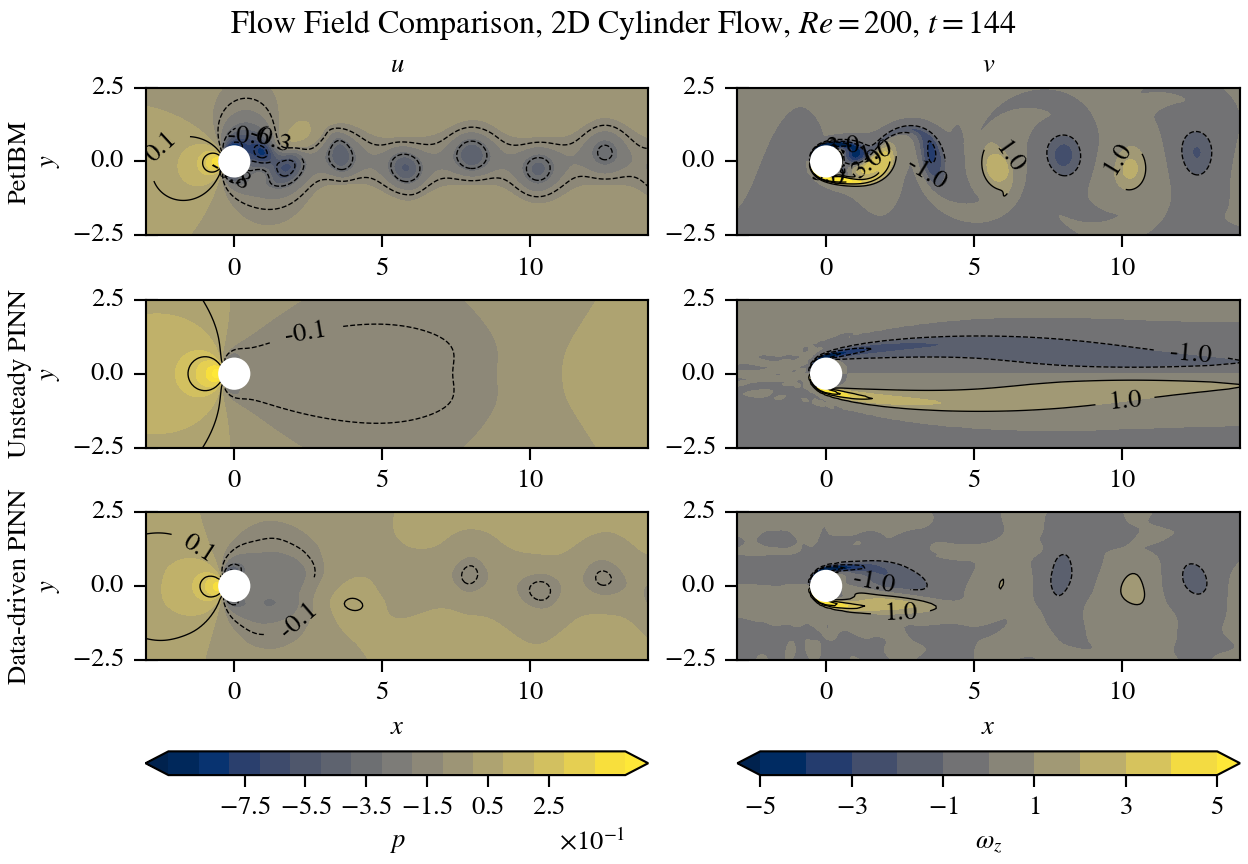
\includegraphics[width=0.9\linewidth]{cylinder-2d-re200/contour-comparison-pwz-t144}
    \caption{2D Cylinder, $Re=200$: flow field comparisons for $p$ and $\omega_z$ at $t=144$ (PetIBM, data-driven PINN, and data-free PINN)}
    \label{fig:cylinder-re200-contour-pwz-t144}
\end{figure}

\begin{figure}[hbt!]
    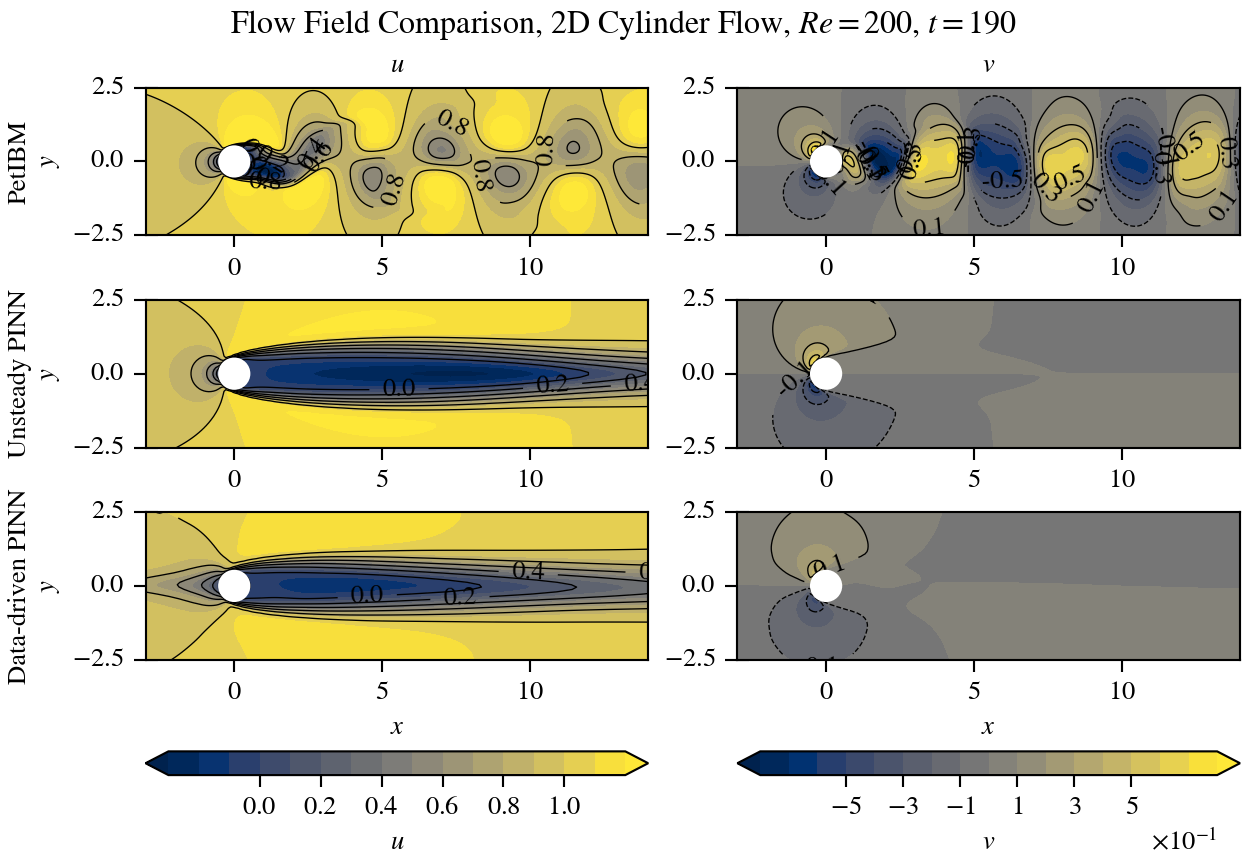
\includegraphics[width=0.9\linewidth]{cylinder-2d-re200/contour-comparison-uv-t190}
    \caption{2D Cylinder, $Re=200$: flow field comparisons for $u$ and $v$ at $t=190$ (PetIBM, data-driven PINN, and data-free PINN)}
    \label{fig:cylinder-re200-contour-uv-t190}
\end{figure}

\begin{figure}[hbt!]
    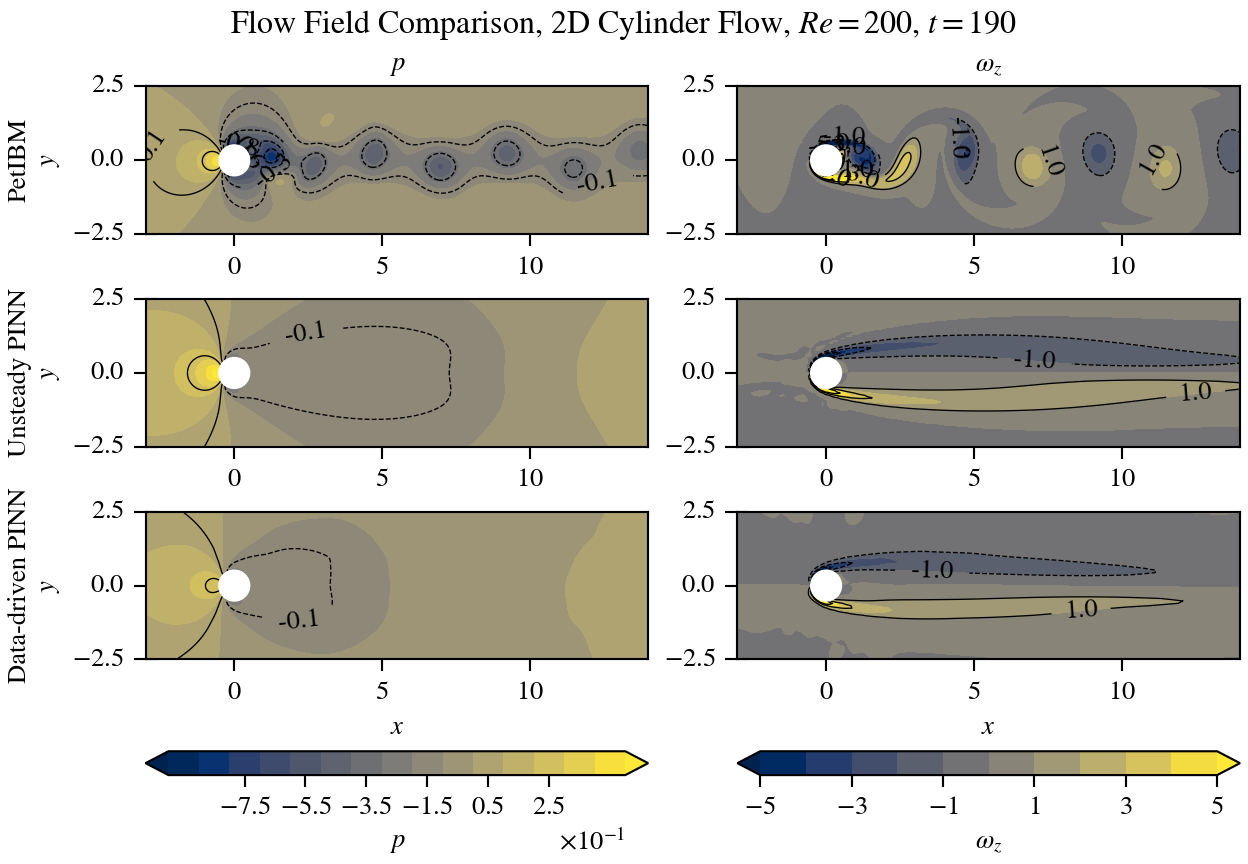
\includegraphics[width=0.9\linewidth]{cylinder-2d-re200/contour-comparison-pwz-t190}
    \caption{2D Cylinder, $Re=200$: flow field comparisons for $p$ and $\omega_z$ at $t=190$ (PetIBM, data-driven PINN, and data-free PINN)}
    \label{fig:cylinder-re200-contour-pwz-t190}
\end{figure}

\clearpage

Figures \ref{fig:cylinder-2d-re200-refined-vort-1} and \ref{fig:cylinder-2d-re200-refined-vort-2} show the vorticity from PetIBM and the data-driven PINN in the vicinity of the cylinder in $t \in [140, 142.5]$, which contains a half cycle of vortex shedding.
These figures compare how vorticity was generated right after we stopped feeding PetIBM data into the data-driven PINN.
These comparisons were expected to shed some light on why the data-free PINN was not able to generate vortex shedding and why the vortex shedding disappeared in the data-driven PINN after $t=140$.

At $t=140$, PetIBM and the data-driven PINN show visually indistinguishable vorticity contours.
This is expected as the data-driven PINN has training data from PetIBM at this time.
At $t=140.5$, a slight difference exists in the result, though nothing seems unphysical.

At $t=141$ and $141.5$ and in PetIBM's results, the main clockwise vortex (the blue circular pattern in the domain of $[1, 2]\times[-0.5, 0.5]$) moves downstream, and it slows down the downstream's $u$ velocity and accelerates the latter's $v$ velocity in $y<0$.
Intuitively, we can treat the main clockwise vortex as a blocker that blocks the flow in $y<0$ and forces the flow move upward.
The net effect is the generation of a counterclockwise vortex at around $x\approx 1$ and $y \in [-0.5, 0]$.
This new counterclockwise vortex further generates a small but strong secondary clockwise vortex on the cylinder surface in $y\in[-0.5, 0]$.
On the other hand, the results of the data-driven PINN at $t=141$ and $t=141.5$ show that the main clockwise vortex becomes more dissipative and weaker, compared to that in PetIBM.
It is possible that the main clockwise vortex is not strong enough to slow down the flow in $y<0$ nor to bring the flow upward.
The downstream flow in $y<0$ (the red arm-like pattern below the cylinder) thus does not change its direction and keeps going straight down in the $x$ direction.

In the results of $t=142$ and $t=142.5$ from PetIBM, the flow completes a half cycle.
That is, the flow pattern at $t=142.5$ is an upside down version of that at $t=140$.
The results from the PINN, however, do not have any new vortices and becomes more like the steady-state flow. 

\begin{figure}[hbt!]
    \centering
    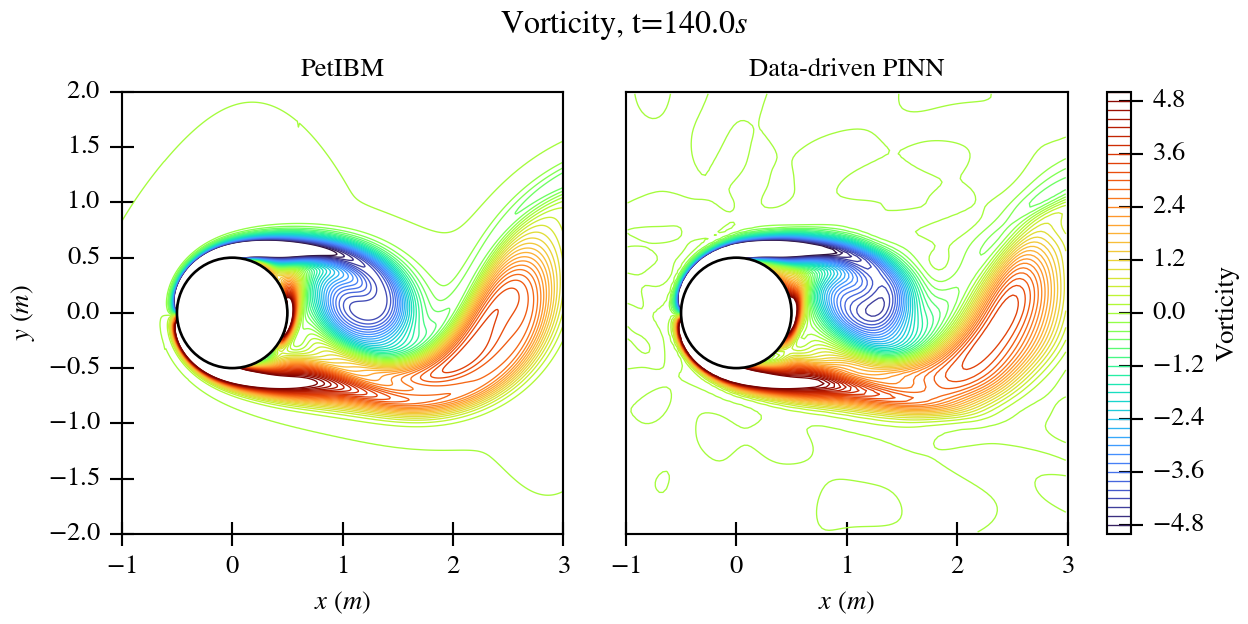
\includegraphics[width=0.925\linewidth]{cylinder-2d-re200/refined/vorticity_z_t140.0}
    \newline
    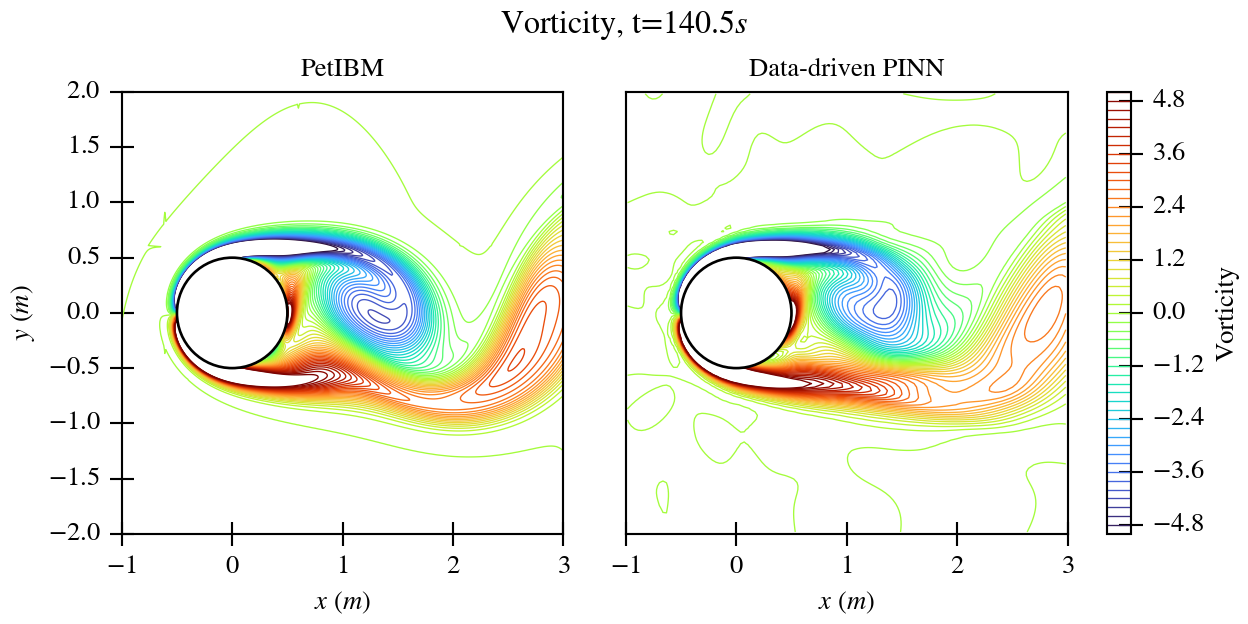
\includegraphics[width=0.925\linewidth]{cylinder-2d-re200/refined/vorticity_z_t140.5}
    \newline
    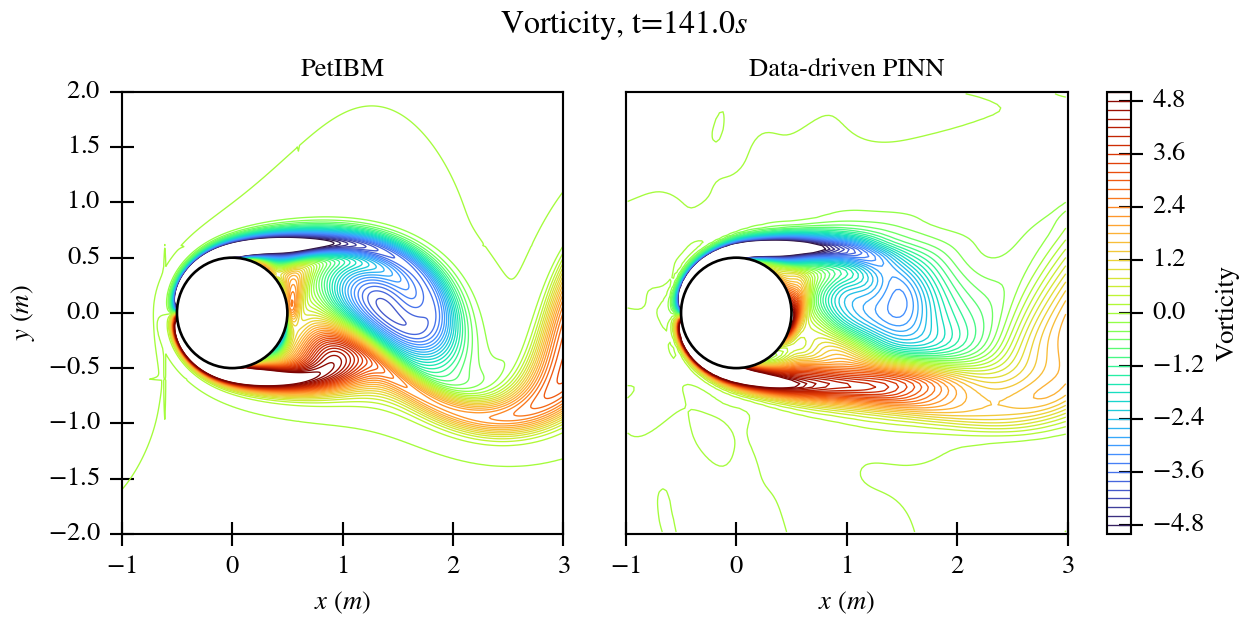
\includegraphics[width=0.925\linewidth]{cylinder-2d-re200/refined/vorticity_z_t141.0}
    \caption{2D Cylinder, $Re=200$: vorticity generation comparison in the vicinity of the cylinder; $t=140$, $140.5$, and $141$ (PetIBM and data-driven PINN)}
    \label{fig:cylinder-2d-re200-refined-vort-1}
\end{figure}

\begin{figure}[hbt!]
    \centering
    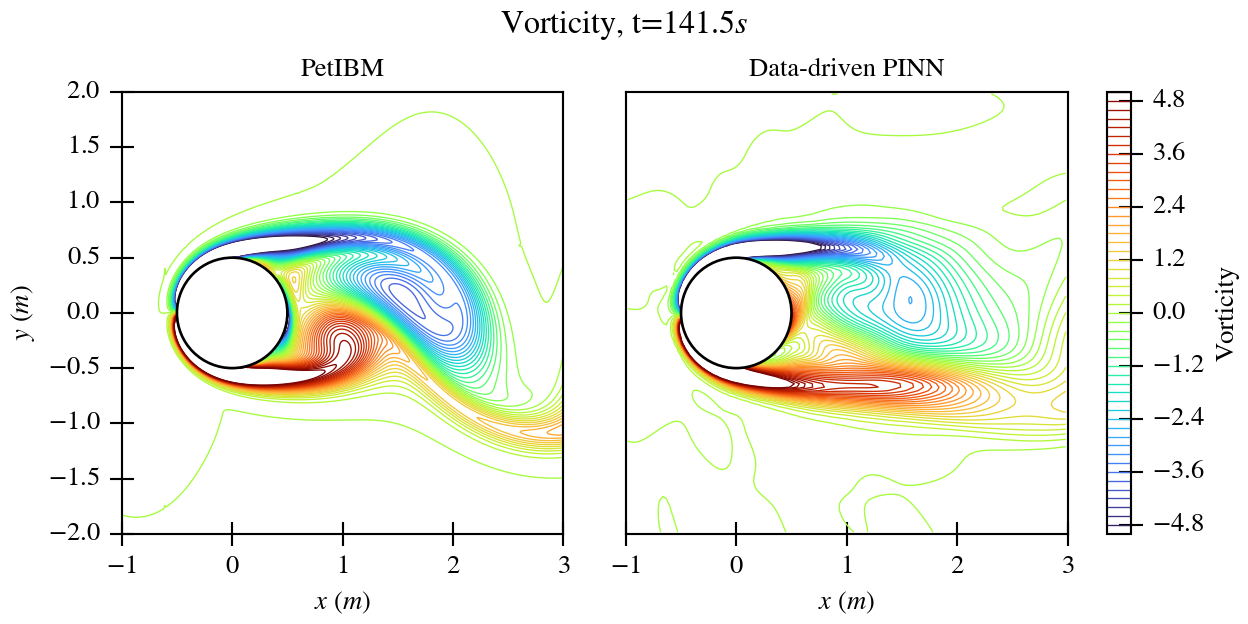
\includegraphics[width=0.925\linewidth]{cylinder-2d-re200/refined/vorticity_z_t141.5}
    \newline
    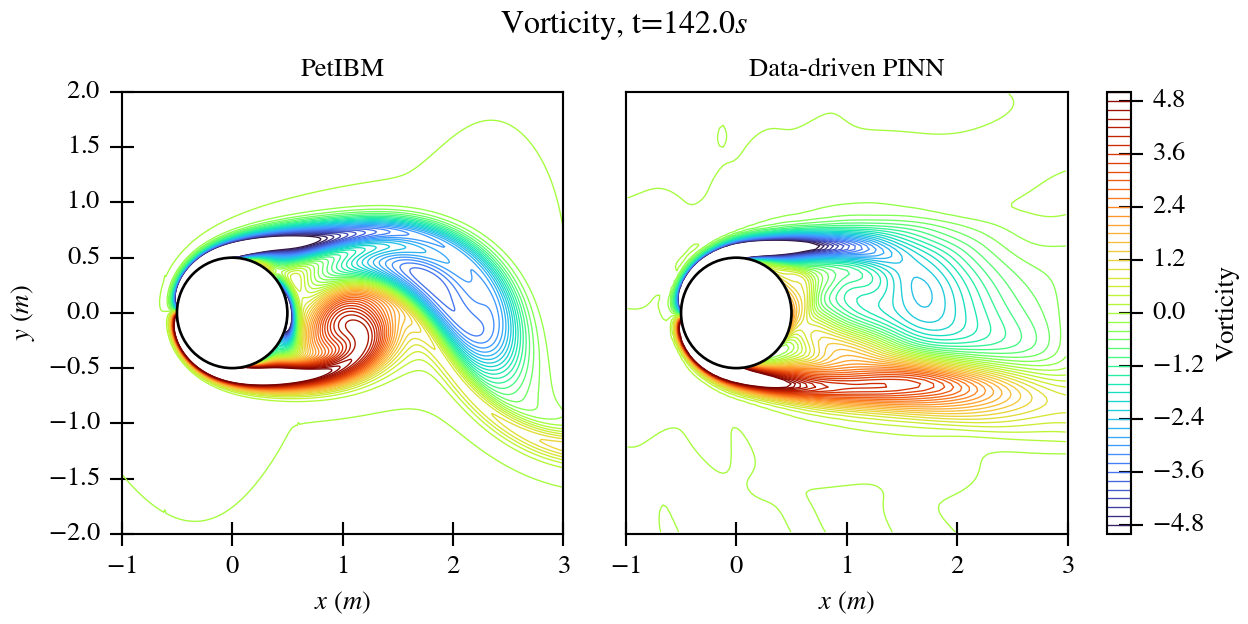
\includegraphics[width=0.925\linewidth]{cylinder-2d-re200/refined/vorticity_z_t142.0}
    \newline
    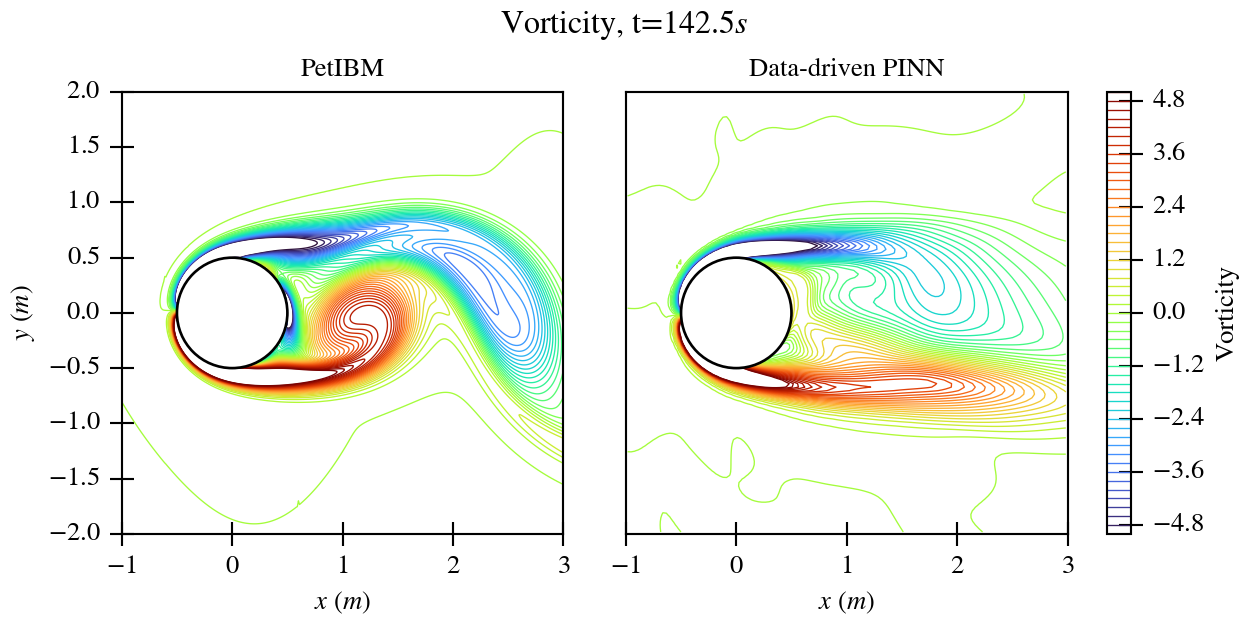
\includegraphics[width=0.925\linewidth]{cylinder-2d-re200/refined/vorticity_z_t142.5}
    \caption{2D Cylinder, $Re=200$: vorticity generation comparison in the vicinity of the cylinder; $t=141.5$, $142$, and $142.5$ (PetIBM and data-driven PINN)}
    \label{fig:cylinder-2d-re200-refined-vort-2}
\end{figure}

Next, we examined the Q-criterion in the same vicinity of the cylinder in $t\in[140, 142.5]$.
Q-criterion is defined as \cite{jeong_identification_1995}:
\begin{equation}
    Q \equiv \frac{1}{2}\left(\lVert \Omega \rVert^2 - \lVert S \rVert^2\right)
\end{equation}
where $\Omega\equiv\frac{1}{2}\left(\nabla\vec{u}-\nabla\vec{u}^\mathsf{T}\right)$ is the vorticity tensor (i.e., rotation rate tensor); $S\equiv\frac{1}{2}\left(\nabla\vec{u}+\nabla\vec{u}^\mathsf{T}\right)$ is the strain rate tensor; and $\nabla\vec{u}$ is the velocity gradient tensor.
A criterion $Q > 0$ identifies the vortex structure in fluid flow, that is, where the rotation rate is greater than the strain rate.
Figures \ref{fig:cylinder-2d-re200-refined-q-1} and \ref{fig:cylinder-2d-re200-refined-q-2} show the Q-criterion results.
We observed that vortices in the PINN are diffusive and could be dissipative.
Moreover, judging by the locations of vortex centers, vortices also move slower in the PINN than in PetIBM.
The edges of the vortices move at a different speed from that of the vortex centers in the PINN.
This might be hinting the existence of the numerical dispersion in the PINN.

\begin{figure}[hbt!]
    \centering
    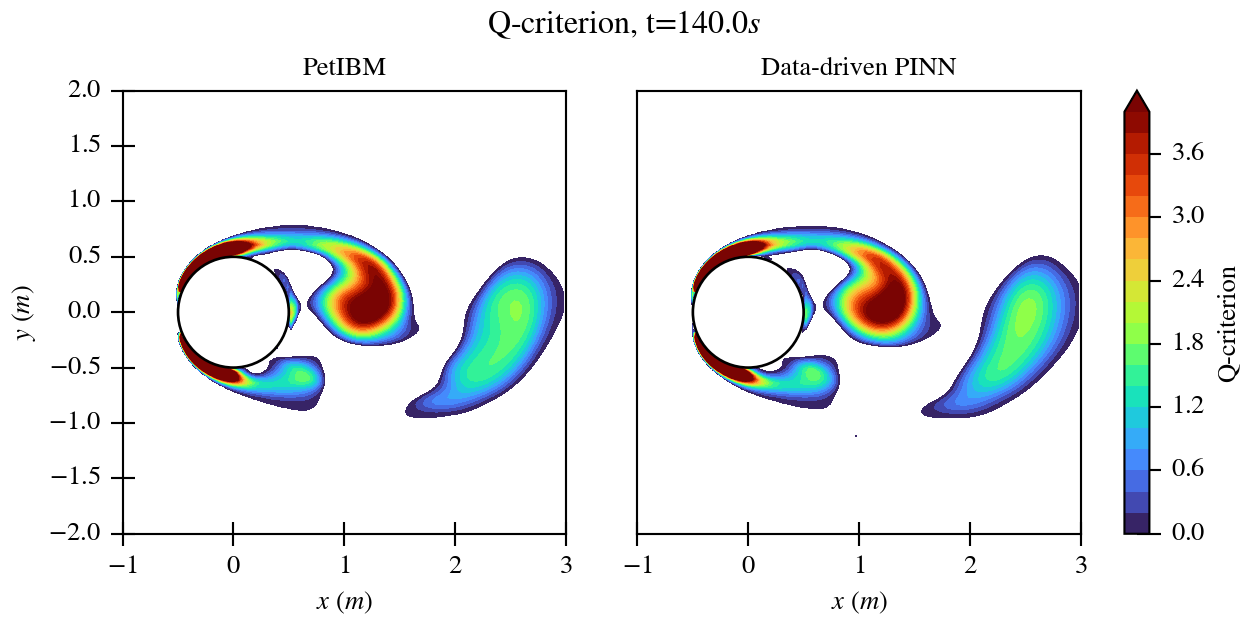
\includegraphics[width=0.925\linewidth]{cylinder-2d-re200/refined/qcriterion_t140.0}
    \newline
    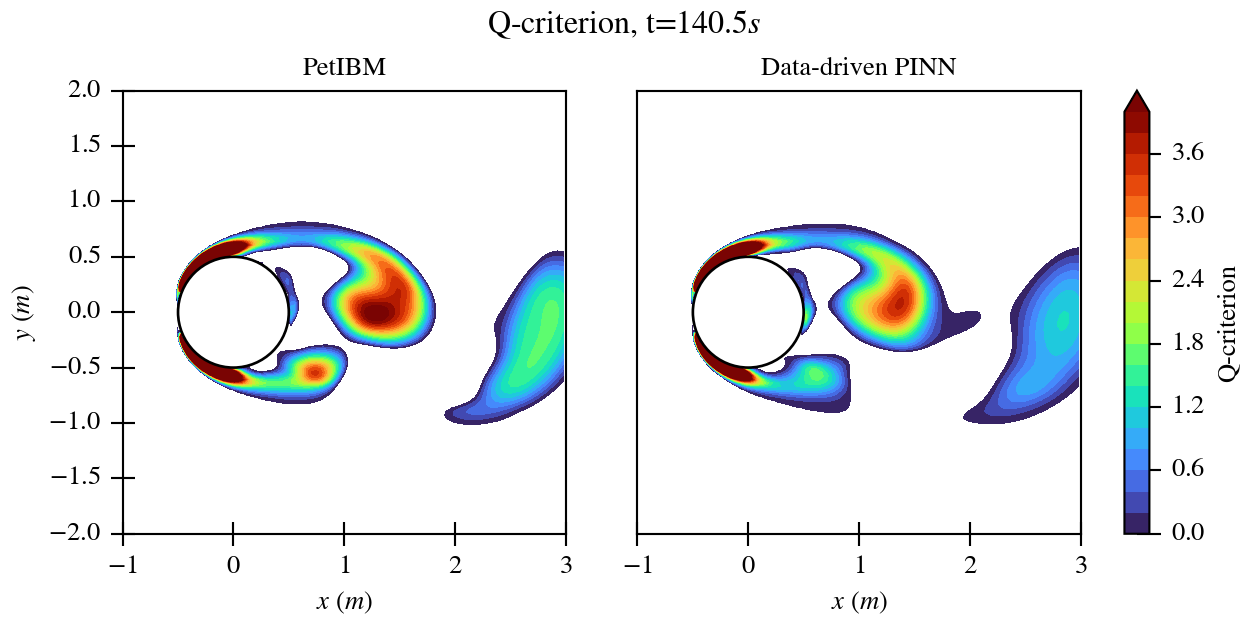
\includegraphics[width=0.925\linewidth]{cylinder-2d-re200/refined/qcriterion_t140.5}
    \newline
    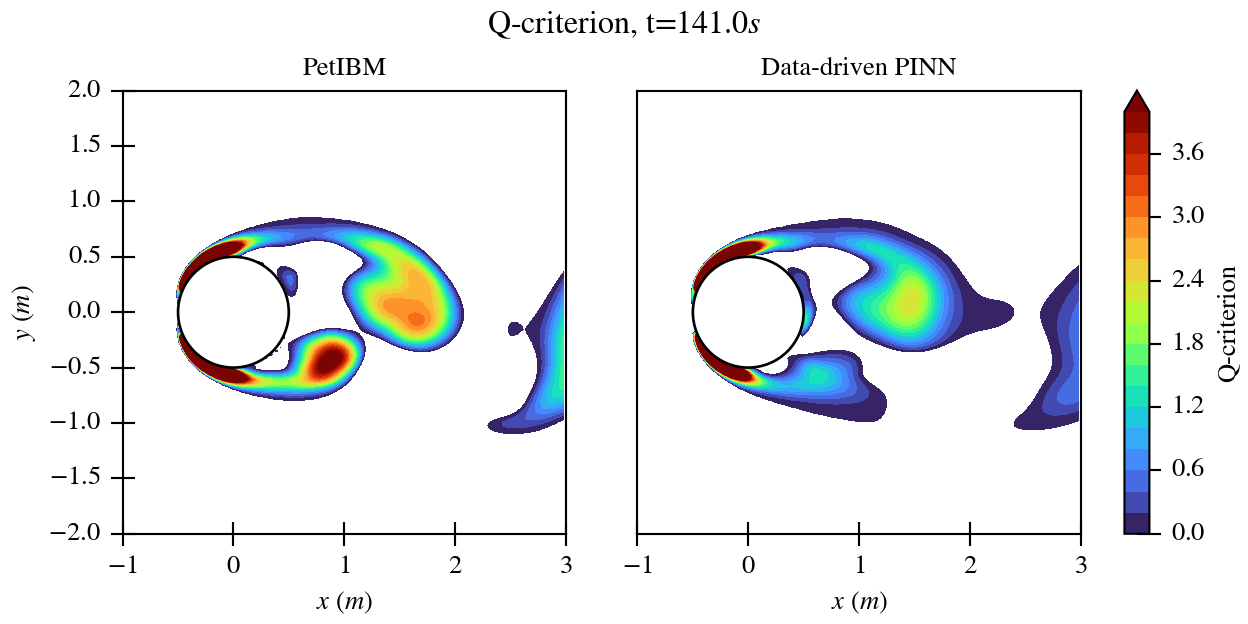
\includegraphics[width=0.925\linewidth]{cylinder-2d-re200/refined/qcriterion_t141.0}
    \caption{2D Cylinder, $Re=200$: Q-criterion in the vicinity of the cylinder; $t=140$, $140.5$, and $141$ (PetIBM and data-driven PINN)}
    \label{fig:cylinder-2d-re200-refined-q-1}
\end{figure}

\begin{figure}[hbt!]
    \centering
    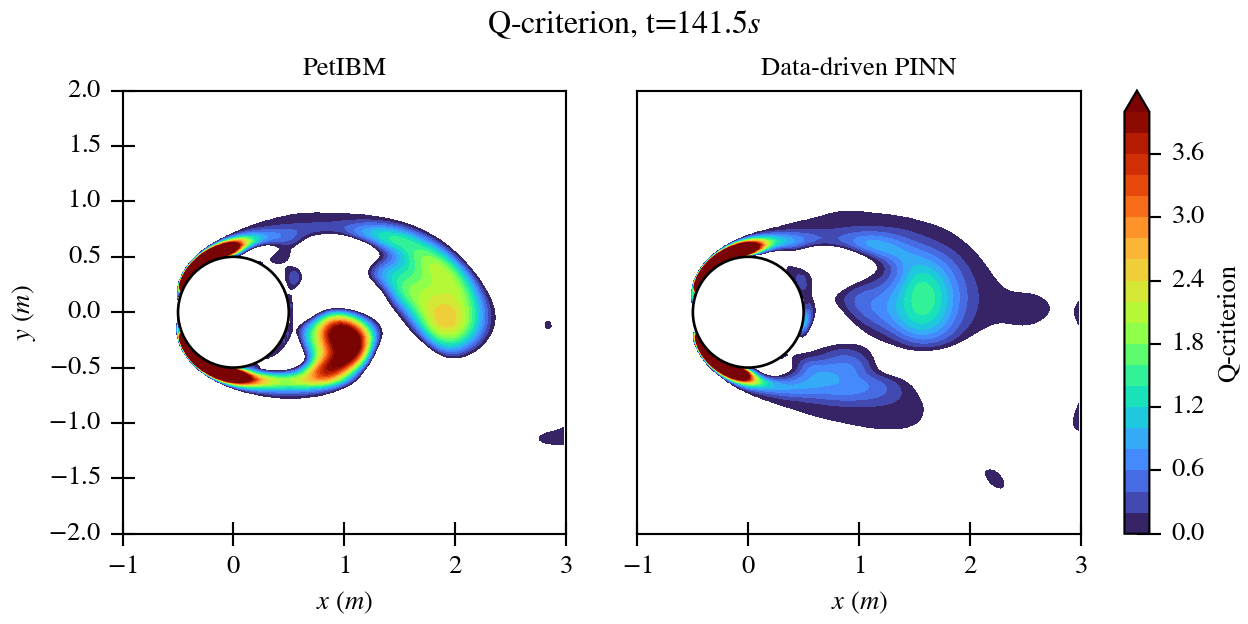
\includegraphics[width=0.925\linewidth]{cylinder-2d-re200/refined/qcriterion_t141.5}
    \newline
    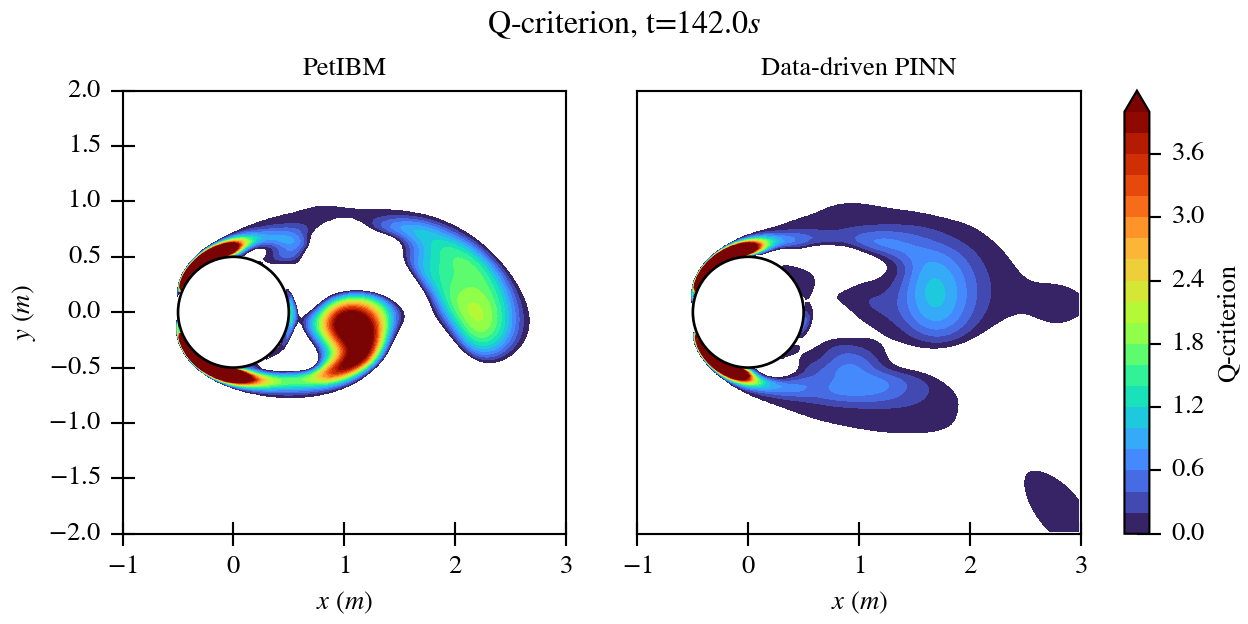
\includegraphics[width=0.925\linewidth]{cylinder-2d-re200/refined/qcriterion_t142.0}
    \newline
    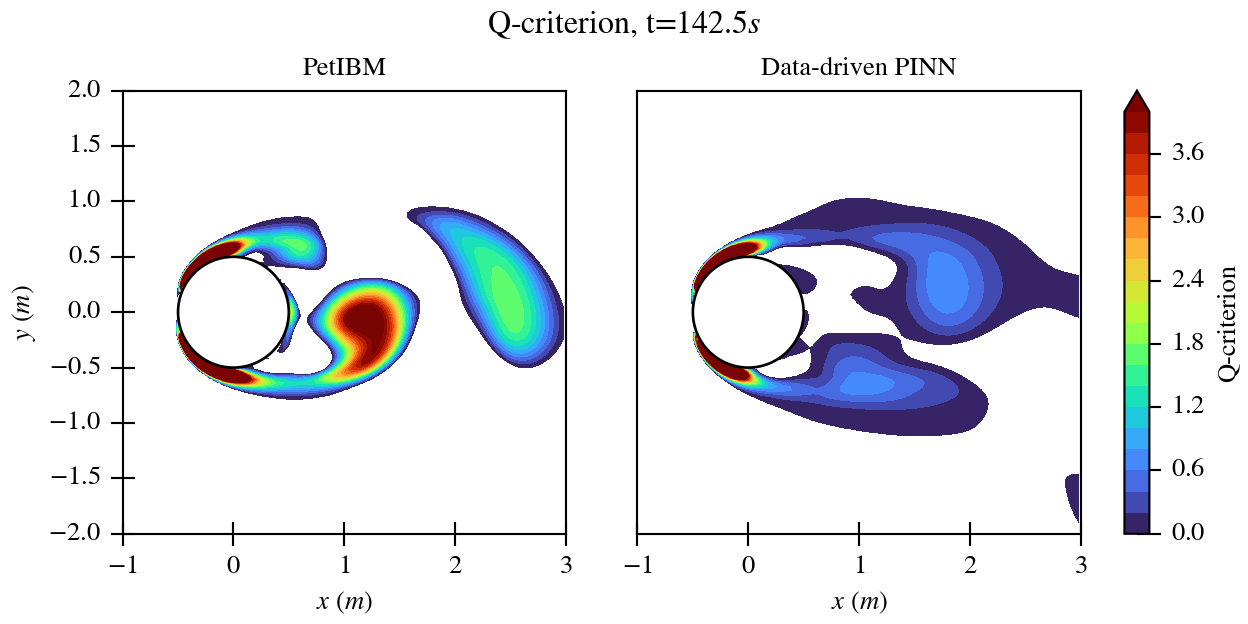
\includegraphics[width=0.925\linewidth]{cylinder-2d-re200/refined/qcriterion_t142.5}
    \caption{2D Cylinder, $Re=200$: Q-criterion in the vicinity of the cylinder; $t=141.5$, $142$, and $142.5$ (PetIBM and data-driven PINN)}
    \label{fig:cylinder-2d-re200-refined-q-2}
\end{figure}

In the next subsection, we would like to apply the spectral analysis to further investigate how information propagate in the temporal direction in the PINN.

\FloatBarrier
% vim:ft=tex
